\subsection{Drift System Implementation}
\label{driftimplementation}

The last chapter conceptionally introduced the \textit{Drift language}
as well as the \textit{Drift Shell}. This chapter will introduce
the current implementation of the \textit{Drift} back-end system,
based on the ideas presented so far.

Both, the Drift language and shell, are heavily influenced
by the idea that most of the semantics of programming for us
programmers is contained within the \textit{names} that are being
used. Which makes it hard to differentiate between which
functionality is defined by the language and which by the shell.

One example of this would be the variable-space which is
defined to consist of names and namespaces only, forming the same
kind of namespace-tree as a traditional UNIX file system.
This tree and variable-space can be walked using the language
keywords \texttt{ls} and \texttt{cd} which are therefor implemented
as shell built-ins.

Furthermore some assumptions and invariants of the underlying
system's behavior have also been sketched, based on the ideas
introduced by chapters \ref{LanguageOfTheSystem} - \ref{bretvictor}.
One example of this would be, that names can be removed from
the pseudo-global namespace emulated by each shell session,
but the data that is referenced by this name needs to be
held on to and made available by the system in case any
running service is still consuming from this data.
So using the concepts of Rich Hickey as introduced in
chapter \ref{LanguageOfTheSystem}, from the user perspective
names behave like places but from the system perspective
data behaves like values.

Another aspect that has already been scratched upon, is the
idea that data should be made observable as soon as it is
available. This is based on the realization that batch
processing is only a special case of stream processing.
In other words: batch data is just streaming data with all
the stream snippets that would otherwise trickle down
over time having already arrived. Therefor any system that
is able to deal with the fact that data might only arrive
as delayed chunks, will naturally be able to deal with a
delay size of 0.

So in order to build a back-end system that supports these
assumptions, one needs to first define the basic tasks of
the front-end (the shell), the back-end and how they interface
with one another. Fig.\ref{system-abstract} shows the
basic idea of how this looks in the current implementation.

\begin{figure}[h]
  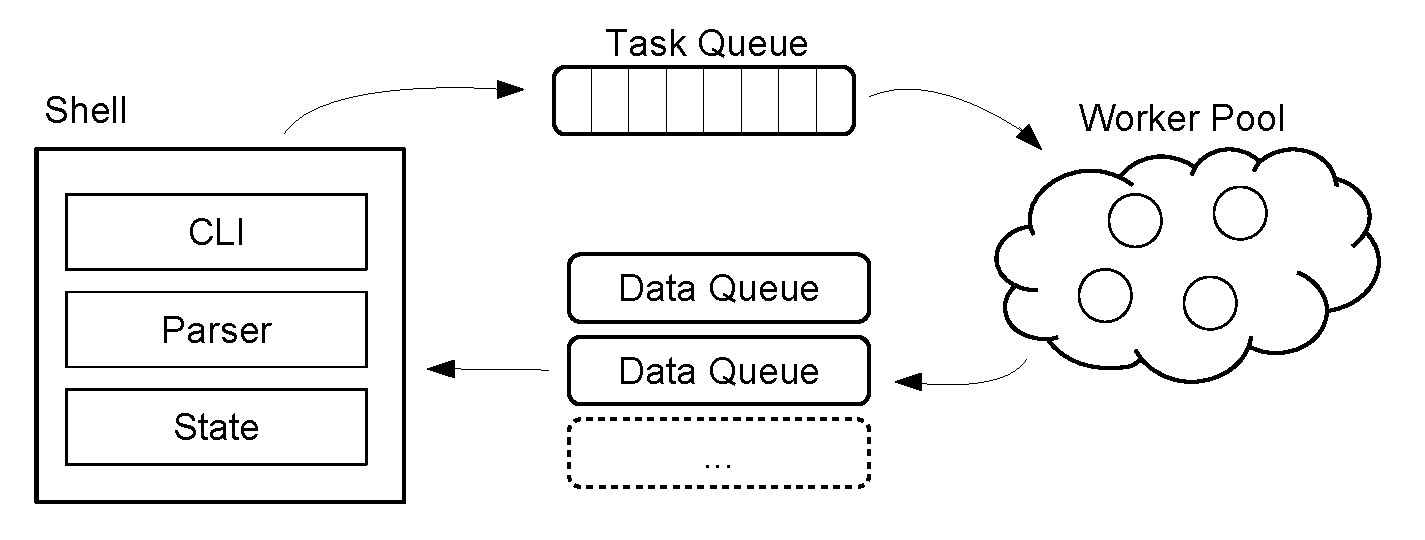
\includegraphics[scale=0.6, keepaspectratio]{system_abstract.pdf}
  \caption{Abstract architecture of the Drift front-end and back-end
           and the interfacing between the two.}
  \label{system-abstract}
\end{figure}

The shell's job is to present the user with a textual interface
and send any valid commands as tasks to the system. Therefor
the shell is \textit{not} part of the system per se. It runs
on the user's machine and connects to the system via network.
This means the user can interface with the system virtually from
anywhere.

Furthermore, as one can see the shell mainly consists of three parts.
All parts and therefor the shell itself are currently implemented
in Java 8 (official version 1.8).
The \textit{command line interface} (CLI) deals with presenting
the shell to the user and handling any input and output from
and to the user. Any input received is passed to the
language parser which was generated using the ANTLR parser
generator (version 4) \cite{antlr}. Additionally in the
parsing layer the shell connects to the service registry which
is not yet shown in the high-level overview of Fig.\ref{system-abstract}.
If any syntactical errors are found or the services do not fit
the specification stored in the service registry, a specific error
message is printed to the screen.

It is important to note however, that in the current implementation
every command entered by the user is fact-checked with the help
of the service registry. This could be optimized by caching any
information retreived about a service in the client shell, therefor
saving round-trips over the network. However, such a caching
infrastructure would, depending on the change rate of the entries
in the service registry, be vulnerable to stale entries. Therefor
some form of cache invalidation or cache coherency protocol would
need to be implemented, updating \textit{all} the client caches
whenever an entry in the service registry changes.
This was considered future work, as will be discussed in the
appropriate chapter, chapter \ref{futurework}.

The third aspect of the shell is the internal state of the session
which consists of two things. A name table that maps the names the
user chose for his session to the names that are used in the system
and the history log for each name.
